In order to refer to our project management, we will talk about the toolings and methods we used,
as summarised in the figure \ref{fig:management:tooling}.

\begin{figure}
    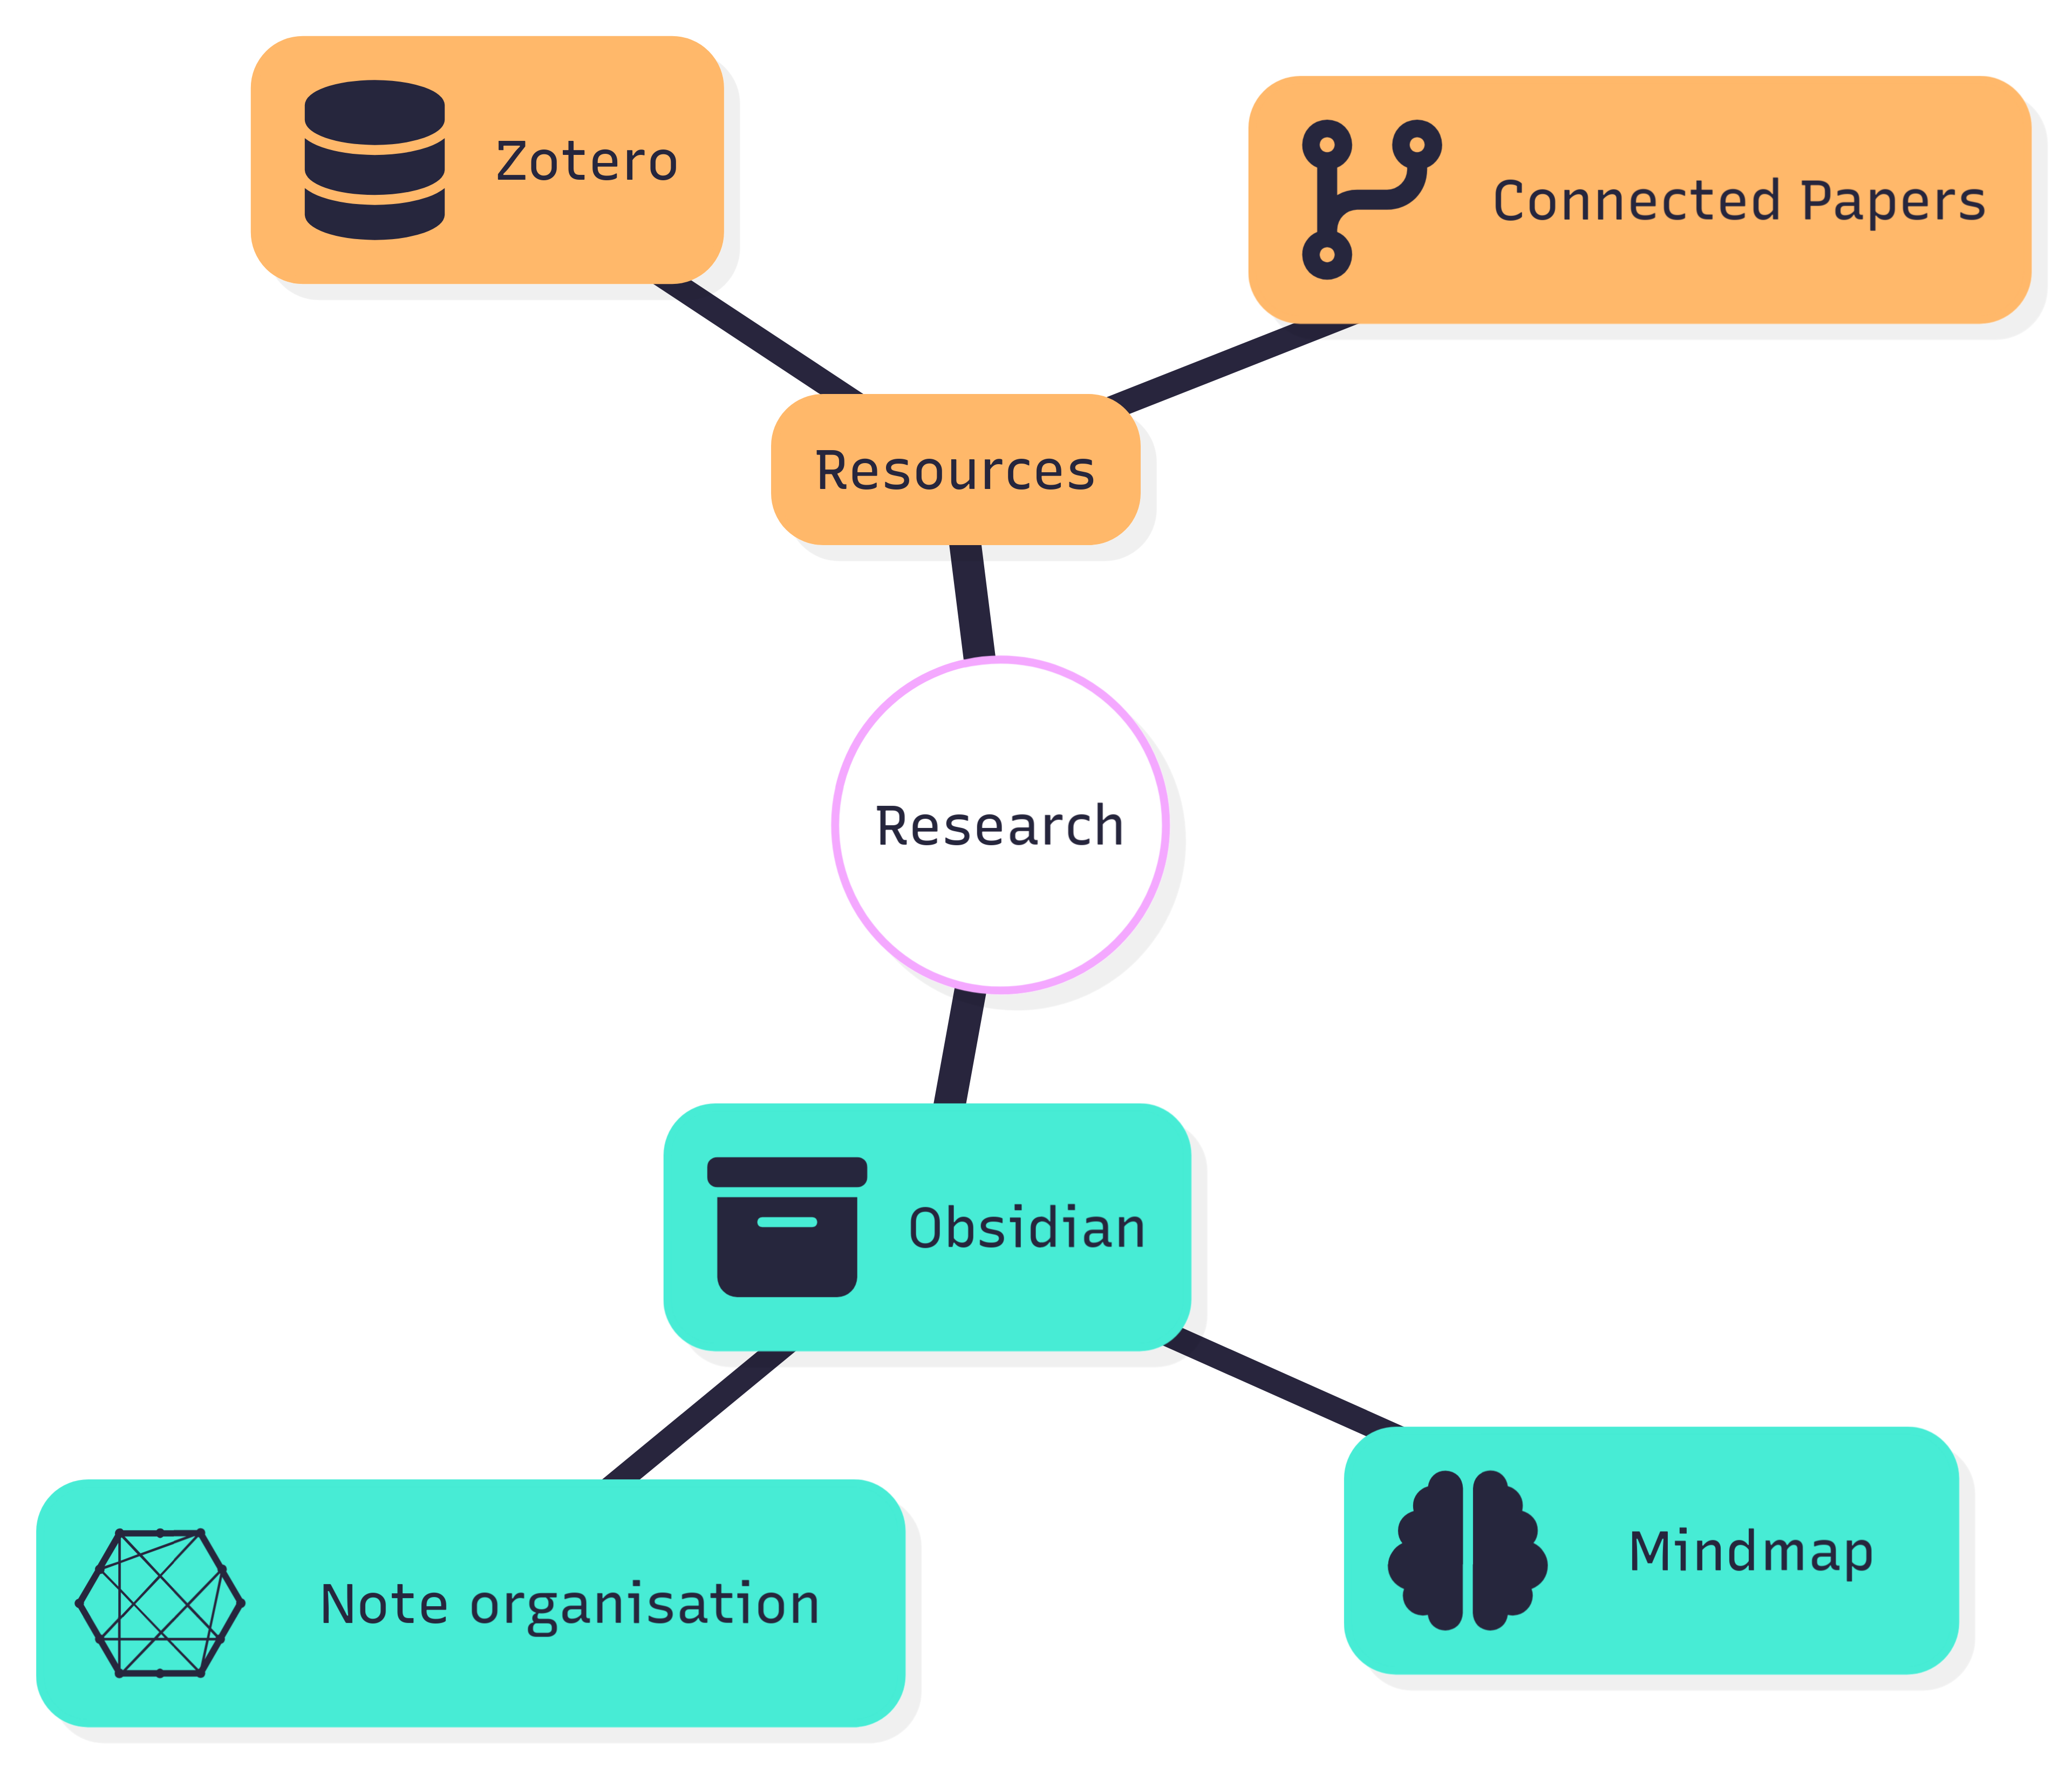
\includegraphics[width=0.45\textwidth]{assets/research-visualisation.png}
    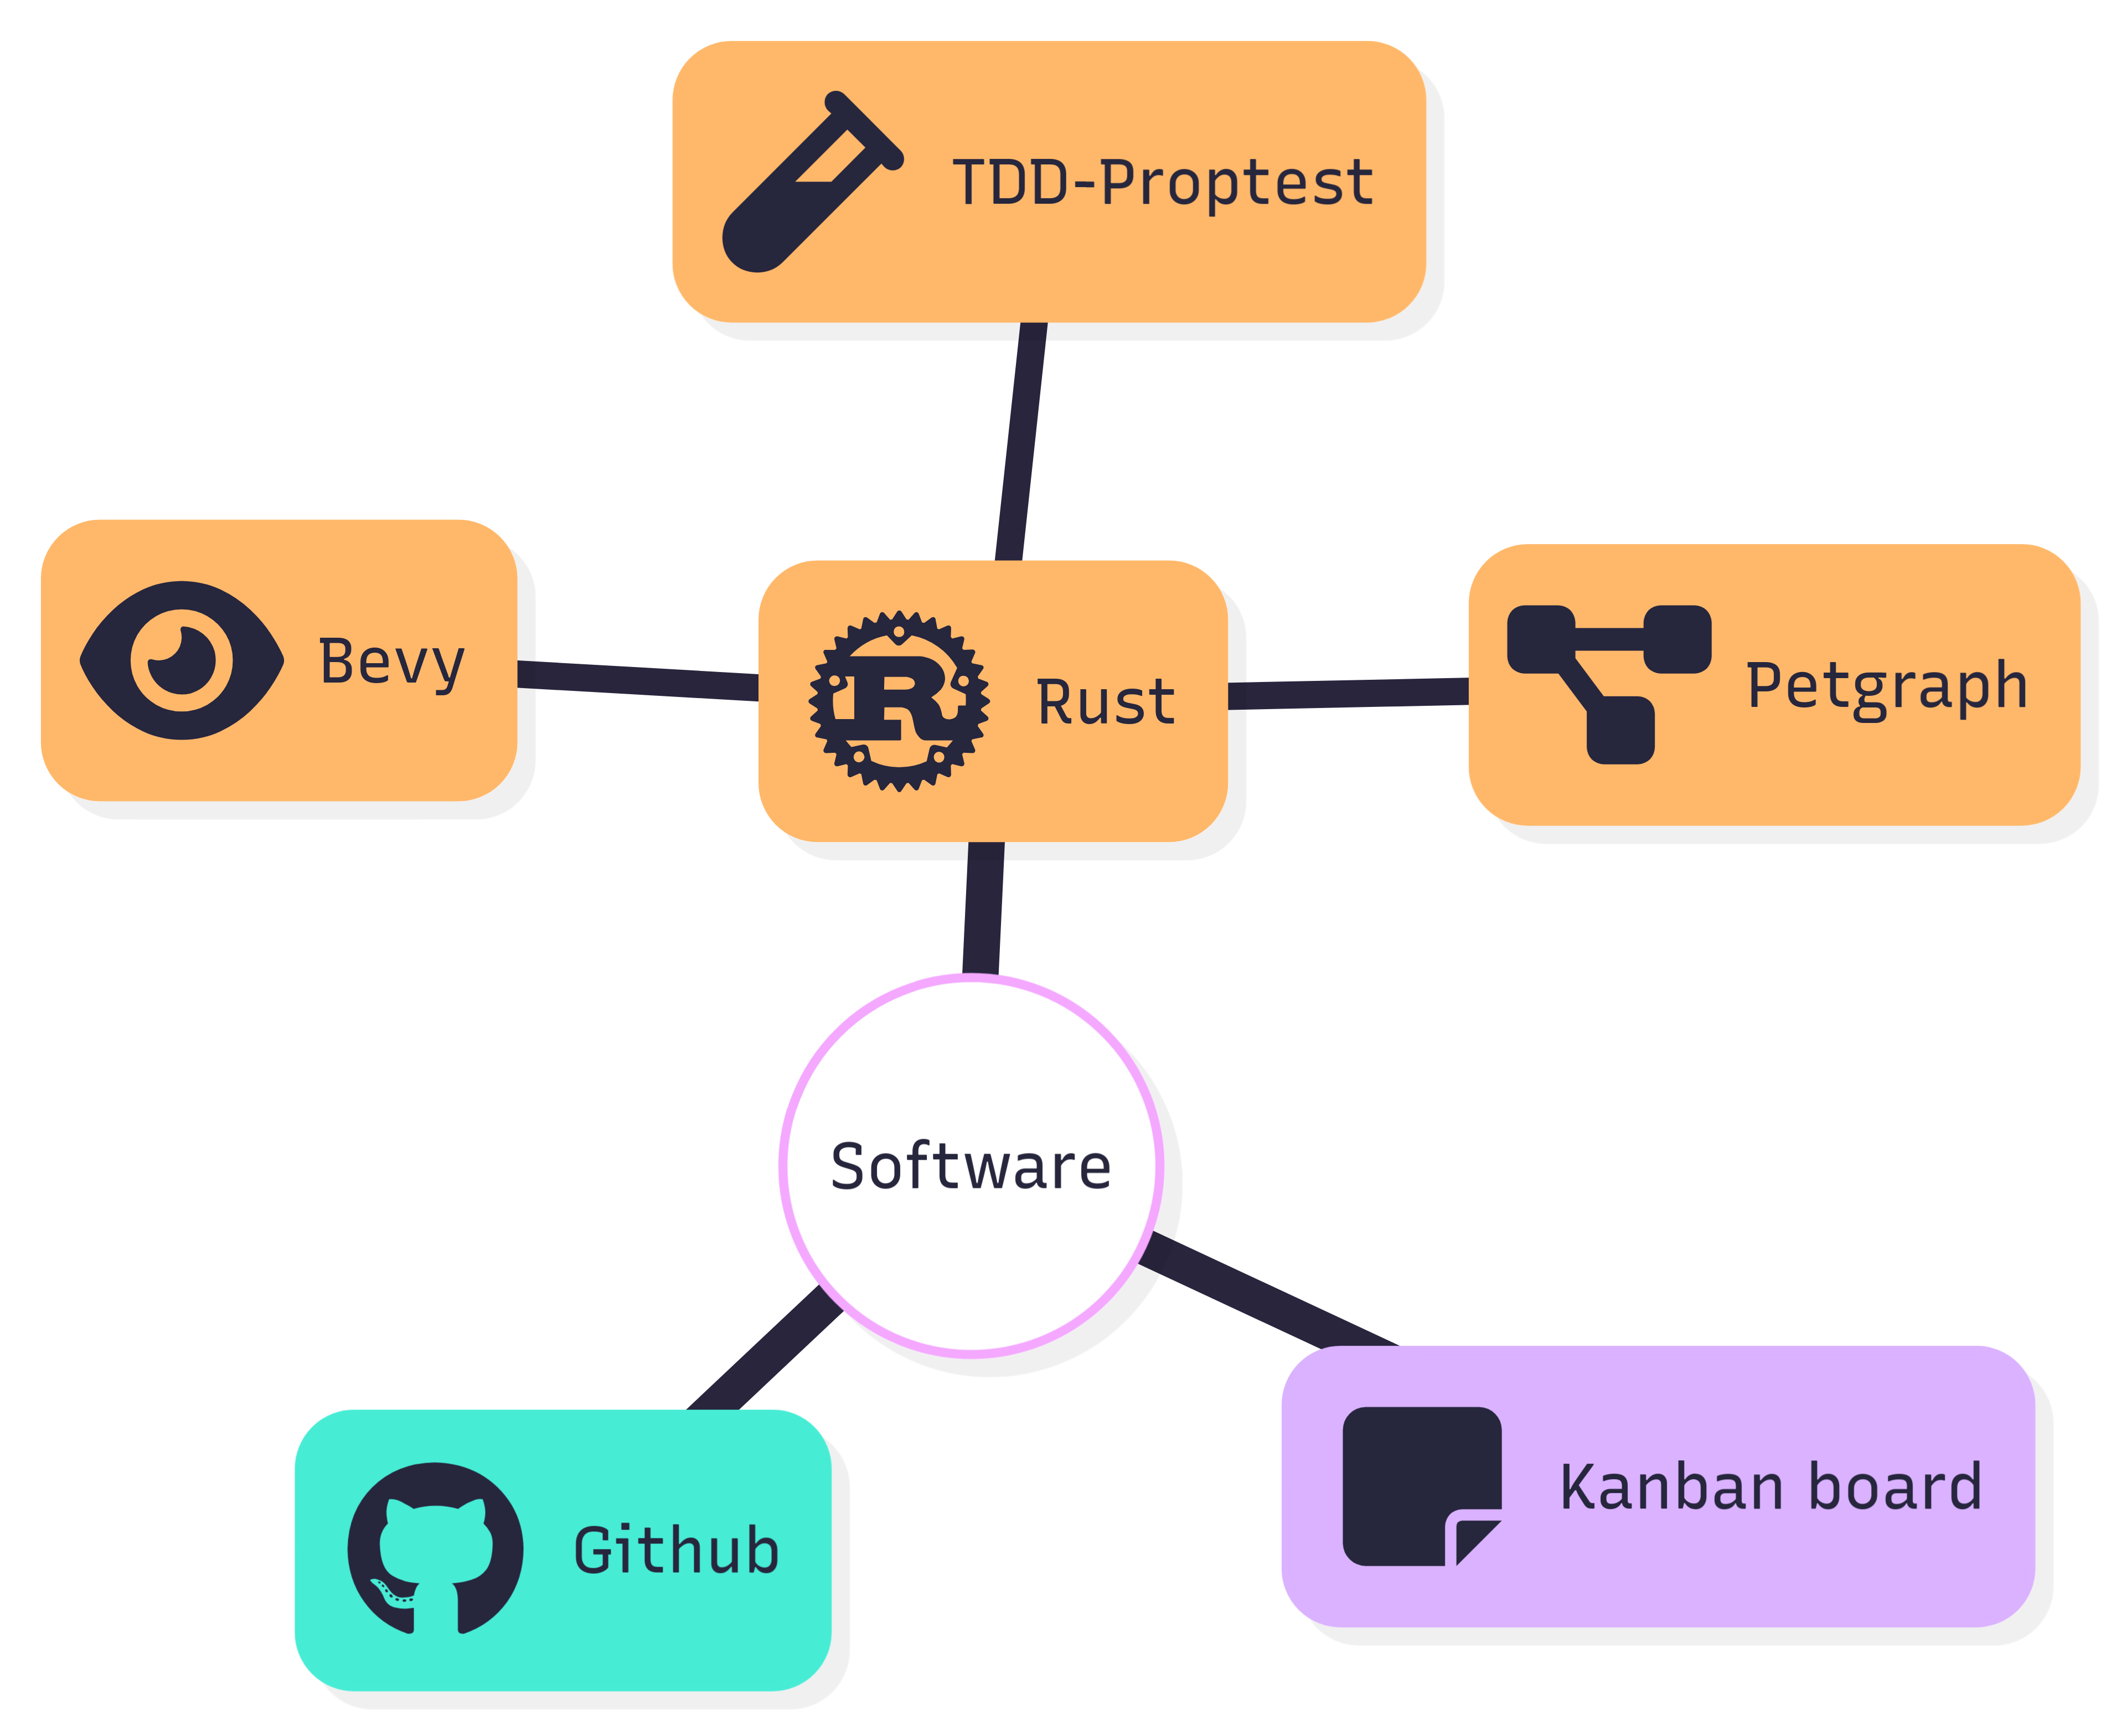
\includegraphics[width=0.45\textwidth]{assets/software-map.png}
    \caption{Tooling}\label{fig:management:tooling}
\end{figure}

Our project also includes the development of a visualisation tool for creation
and verification of several \textsc{PureCircuit} instances. We will use the
figure \ref{fig:soft:workflow} for main reference. We opted with \textit{Rust},
as the main language of development, due to its high and low level features.
From the one hand, \textit{Rust} can efficiently handle memory allocation safely
with its clever usage of the Borrower-Ownership framework. Conversely, it implements
a strongly typed system with help of generics, associated types and algebraic types
allowing us to create a versatile and compact library. Given the above, we utilise
techniques such as \texttt{Proptest}, where we create strategic randomized tests
that check whether  function follows an expected property. On the other hand
we make use of \texttt{Petgraph}, which is a sophisticated library that handles
graph-like structures in \textit{Rust}.


For visualisation we decided to go with \textit{Bevy}. \textit{Bevy} is a
game engine that uses the \textit{ECS} software achitecture. A general
workflow of an \textit{ECS} system can be described as such: a state 
contains entities, each of which is composed of components or properties.
A system is a specialised method that gathers entities based on their components
and describes an interaction between them. This whole process can be visualised
in the figure \ref{fig:soft:ecs-workflow}


\begin{figure}[h!]
    \centering
    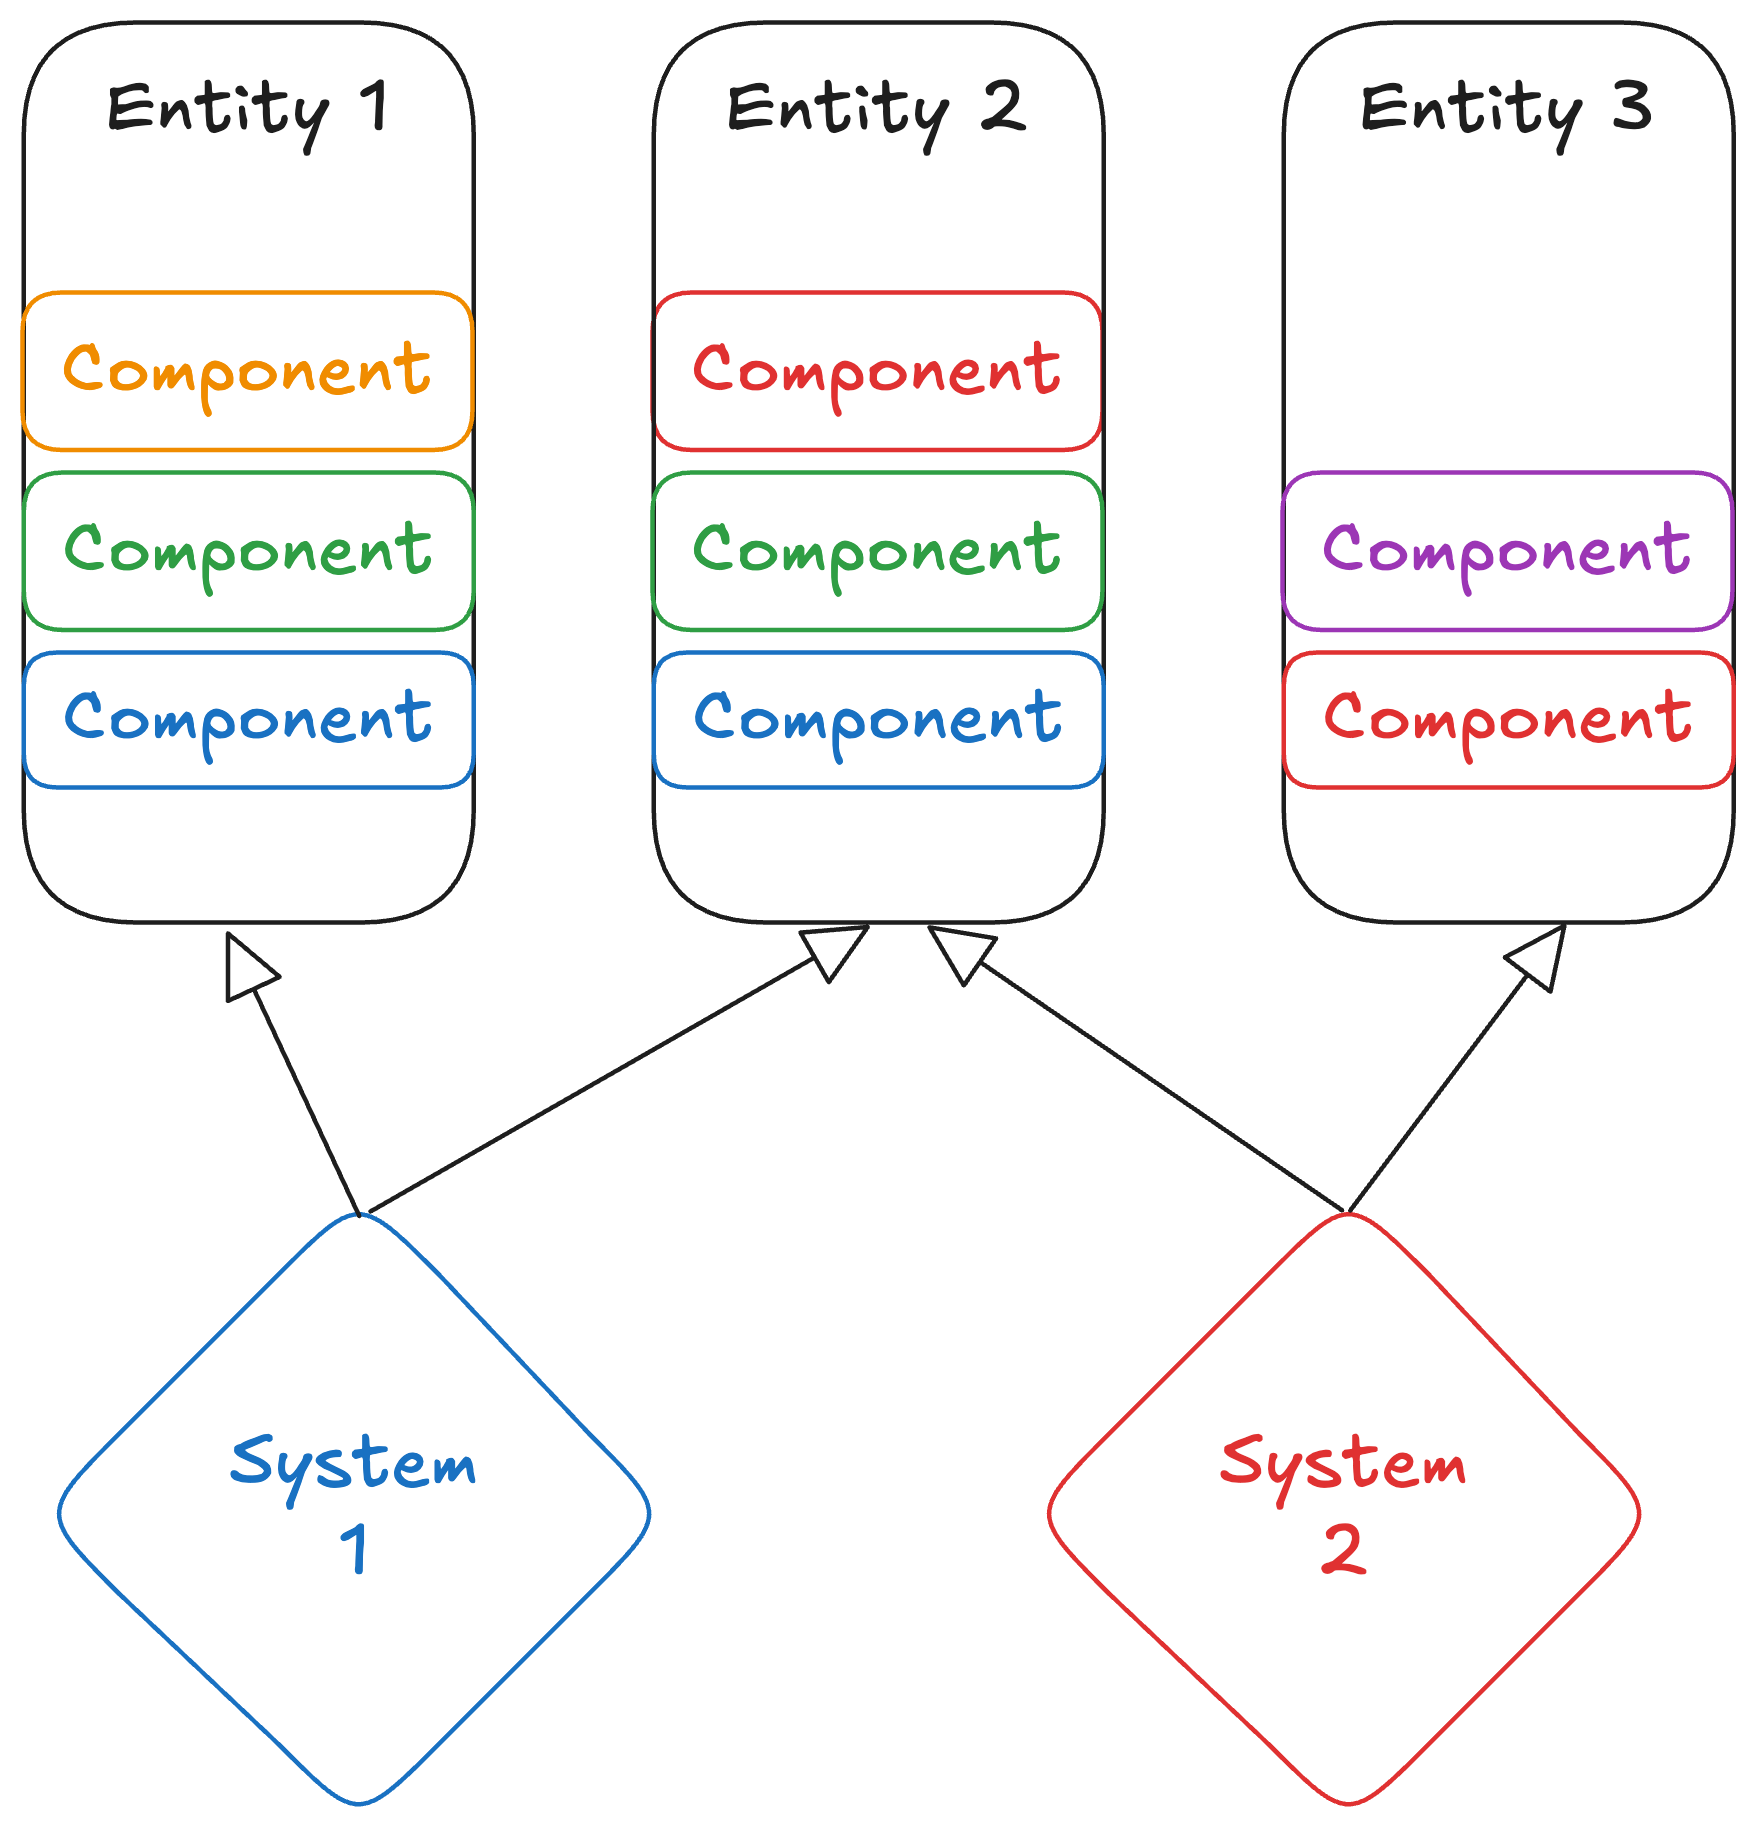
\includegraphics[width=0.35\textwidth]{assets/ECS-visualisatoin.png}
    \caption{ECS workflow visualisation}
    \label{fig:soft:ecs-workflow}
\end{figure}




